\section{Association Analysis}
\subsection{Introduction (*)}

L'analisi di associazione aiuta a comprendere il concetto di causalità di variabili: dati certi valori di attributi cosa posso dire del valore di un altro attributo?

Le regole associative permettono di prendere delle scelte molto operative in diversi ambiti, in particolare in quello che viene chiamato il problema del \textit{market basket analysis}. 
Il problema del carrello tratta il posizionamento di prodotti in un negozio. \`E noto che all'acquisto di un certo prodotto si tende ad acquistare altri prodotti connessi, quindi si cercano queste associazioni basandosi sul carrello della spesa dei clienti (appunto market basket) per poi capire come impostare la disposizione sugli scaffali.

\textbf{Obiettivo}: identificare quali siano gli \textbf{item associati} per poter prendere delle decisioni. In sostanza si generano \textbf{Regole associative} formate da coppie di insiemi \textit{antecedente} e \textit{conseguente}.

es. \{Beer\} $\rightarrow$ \{swiss cheese\} 

\quad \{antecedente\} $\rightarrow$ \{conseguente\}\\
\textit{\`E molto importante ricordare che questo tipo di analisi serve a trovare associazioni non causalità.} \\
L'analisi si basa sullo studio di due diversi dataset:
\begin{itemize}
	\item \textit{Product set:} contiene informazioni legate ai prodotti come il nome e il prezzo
	\item \textit{ransaction set:} contiene informazioni legate agli acquisti dei clienti, ogni record corrisponde ai prodotti presenti nel carrello del cliente
\end{itemize}

Si organizza il dataset delle transazioni in formato binario, ovvero ogni colonna indica se in una data transazione un certo prodotto sia o meno presente.

\begin{figure}[H]
	\centering
	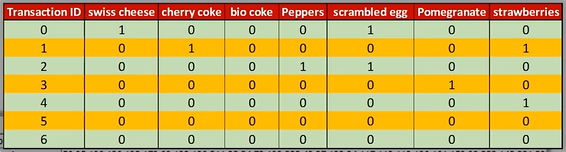
\includegraphics[height=0.25 \linewidth]{association/pict/transaction_set_bin.png}
	\caption{Esempio: transaction set binarizzato}
\end{figure}
Di seguito viene proposto un elenco delle grandezze fondamentali per la trattazione di un problema di associazione; in particolare, si considerino:
\[I = \{i_1, i_2,...,i_d\}\] 
Il set di tutti gli item nel market basket

\[T = \{t_1,t_2,...,t_N\}\] 
L'insieme di tutte le transazioni

\begin{defn}
	Si definisce \textbf{Itemset} una collezione di zero o più item.
\end{defn} 
\begin{defn}
	Si definisce \textbf{K-Itemset} un itemset che contiene k item .
\end{defn}
\begin{defn}
	Si definisce \textbf{empty set} l'itemset che non contiene alcun elemento.
\end{defn}
\begin{defn}
	Si definisce \textbf{transaction width} il numero di item presenti in una transazione
\end{defn}
	 
Una transazione $t_j$ contiene l'itemset $X$, se $X$ è un sottoinsieme di $t_j$.

\begin{defn}
	Si definisce \textbf{Support count} il numero di transazioni che contentono uno specifico itemset.

\[ \sigma(X) = |\{t_i | X \subseteq t_i, t_i \in T\} \]
\end{defn}

\begin{defn}
Una \textbf{regola di associazione} è definita come:

$X \rightarrow Y$

dove $X$ e $Y$ sono itemset disgiunti ($X \cap Y = \emptyset$).
\end{defn}
Una regola viene valutata in termini di \textit{supporto} e di \textit{confidenza}.

\begin{defn}
	Si definisce \textbf{Support} la seguente grandezza: 
	
	\[s\{x \rightarrow Y\} = \frac{\sigma(X \cup Y)}{N}\]
\end{defn}
Come si può notare il supporto serve a determinare quanto spesso una regola è  applicabile dato un data set.
\begin{defn}
	Si definisce \textbf{Confidence} la seguente espressione: 	
	\[c\{x \rightarrow Y\} = \frac{\sigma(X \cup Y)}{\sigma(X)}\]
\end{defn}
\`E evidente che determina quanto frequente sia Y presente in una transazione che contiene X.

Di seguito un \textbf{esempio} che fa comprendere come vengano utilizzate queste grandezze. 
\[X = \{swiss cheese, cheddar\} \quad Y = \{diet coke\}\]
Si assuma che:
\begin{itemize}
	\item $\sigma(x) = 8$ (support count)
	\item $N = 20$ (numero di transazioni)
	\item $\sigma(x,y) = 6$ 
\end{itemize}
Allora il support e la confidence della regola $X \rightarrow Y$ sono:

\[s\{X \rightarrow Y\} = \frac{\sigma(X \cup Y)}{N} = \frac{6}{20} = 0.3\]

\[c\{x \rightarrow Y\} = \frac{\sigma(X \cup Y)}{\sigma(X)} = \frac{6}{8} = 0.75\]

Le \textbf{motivazioni} che spingono ad utilizzare una grandezza come il supporto sono le seguenti:
\begin{itemize}
	\item Se troppo basso potrebbe esserci un'associazione casuale
	\item Potrebbe non valere la pena seguire associazioni che si applicano in modo poco significativo dal punto di vista dei profitti 
\end{itemize}

\textit{Il concetto di supporto è utilizzato per eliminare regole non desiderate e condivide interessanti proprietà che possono essere sfruttate per la ricerca di regole associative efficaci.
La confidenza è molto importante perché misura l'affidabilità dell'inferenza} e:
\begin{itemize}
	\item Un' alta confidenza significa che Y sarà molto presente in transazioni con X .
	\item Si stima la probabilità condizionata di Y dato X.
\end{itemize}
\begin{defn}
Si definisce \textbf{Association Rule Mining Problem} il problema che è formalmente definito come: dato un set di transazioni T, trovare tutte le regole con $support \ge minsup$ e $confidence \ge minconf$, dove $minsup$ e $minconf$ sono i threshold corrispondenti alle due misure.
\end{defn}
Ci sono diversi metodi per risolvere il problema, il primo che viene considerato è il seguente: \\
\textit{Approccio a forza bruta} di association rule non è molto praticabile in quanto i tempi di computazione aumentano in modo esponenziale: 

\[R = 3^d - 2^{d+1} + 1\]

\begin{figure}[H]
	\centering
	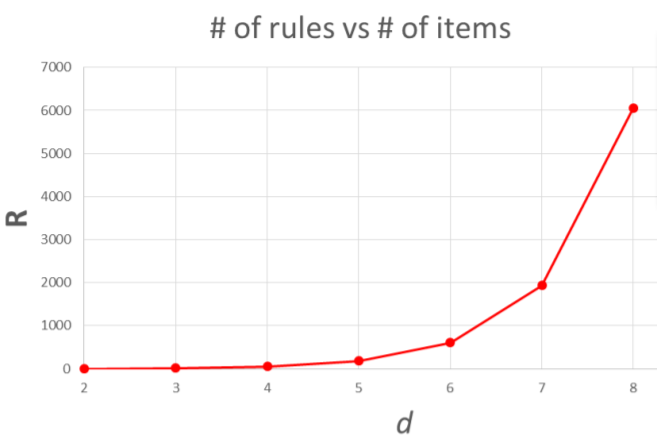
\includegraphics[height=0.4 \linewidth]{association/pict/brute_force.png}
	\caption{Numero di regole calcolate in base al numero di itemset}
\end{figure}

Una strategia comunemente adottata in molti algoritmi è quella di decomporre il problema in 2 grandi supertask:
\begin{itemize}
	\item\textit{Generazione dei frequenti itemset}: vengono specificate tutte e sole quelle regole per cui il supporto è maggiore del $minsup$, gli itemset generati sono chiamati \textbf{Frequent Itemset}
	\item \textit{Generazione delle regole}: vengono estratte tutte le regole con alta confidenza (maggiore di $minconf$) dai Frequent Itemset trovati precedentemente, queste regole vengono chiamate \textbf{Strong Rules}
\end{itemize}
La complessità maggiore è richiesta dalla generazione dei Frequent Itemset.


\subsection{Rule Extraction}

Per comprendere l'inefficienza della generazione con l'approccio forza bruta si faccia riferimento al seguente esempio:
\begin{figure}[H]
	\hspace{-0.7 cm}
	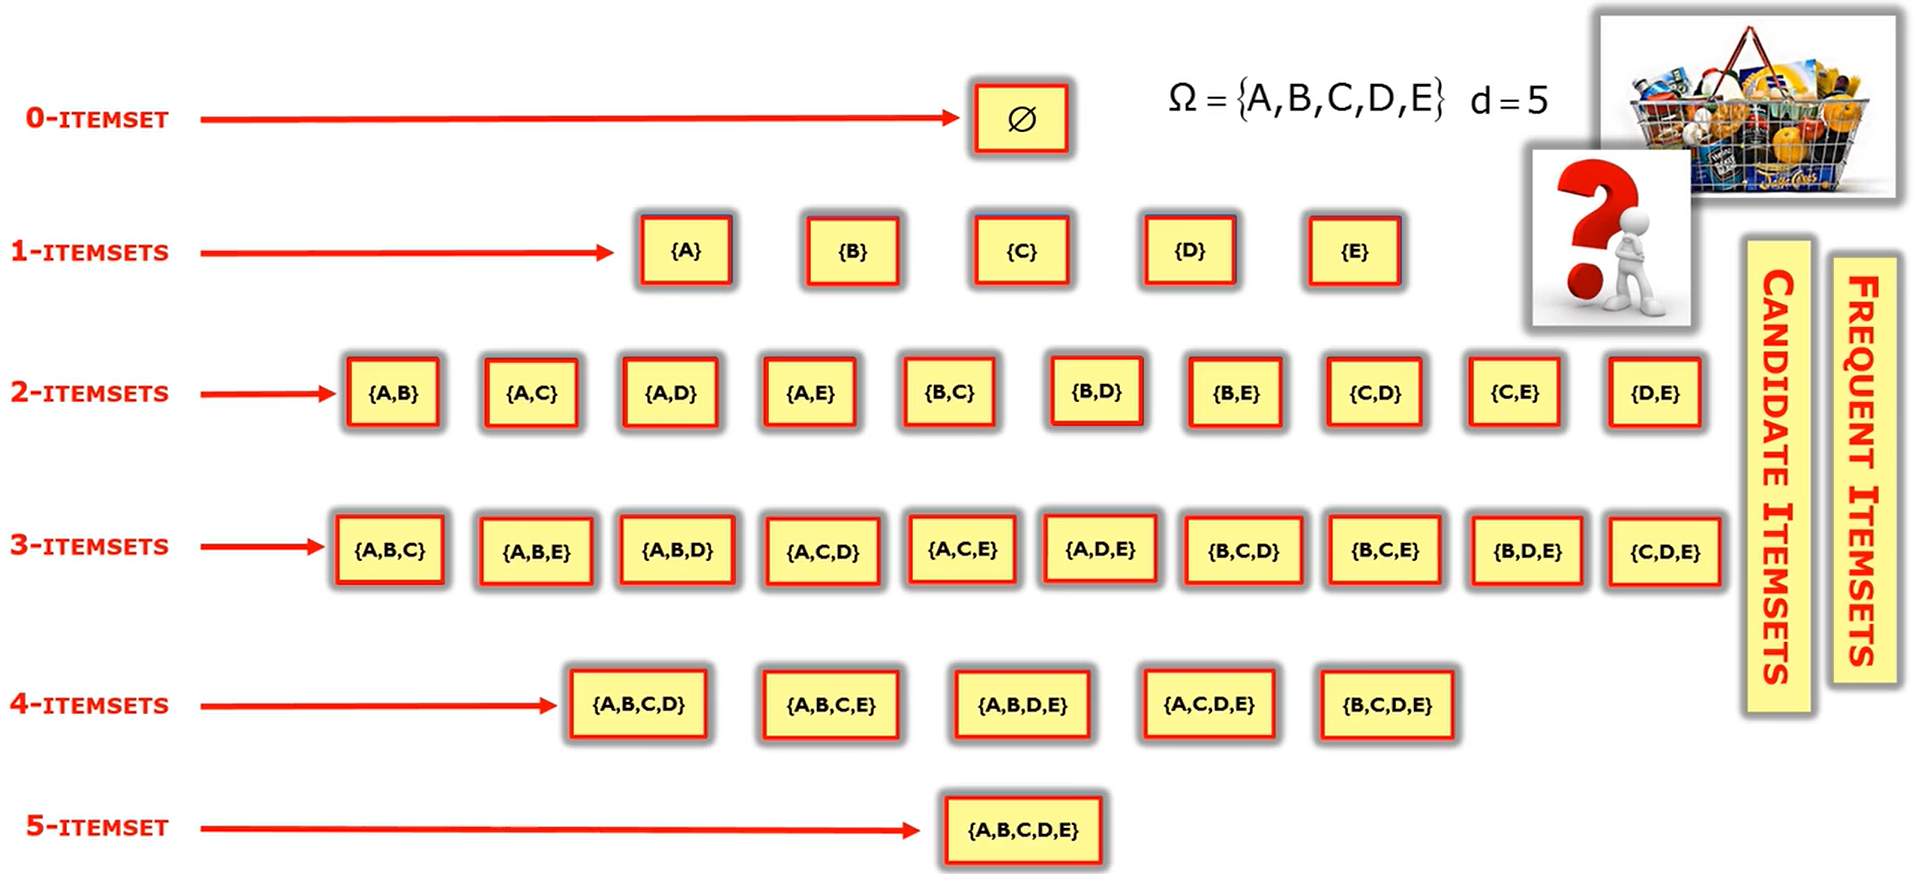
\includegraphics[height=0.5 \linewidth]{association/pict/k-itemset.png}
	\caption{k-itemset brute-force}
\end{figure}
\begin{defn}
	Si definisce \textbf{Candidate Itemset} l'insieme di tutti gli itemset che possiamo formare. 
\end{defn}
Per come sono definiti questi insiemi potranno contenere un numero diverso di itemset; nel nostro caso il numero di itemset candidato è: 
\[M = 2^{d} - 1 = 2^5 -1 = 31\]

Come si può notare è presente un sistema a doppio cono tipico delle distribuzioni binomiali. Una volta che sono stati considerati tutti si è interessati solo ai più frequenti. \\
Se si usasse la forza bruta bisognerebbe calcolare per ogni itemset candidato il suo support count, e vedere se il suo supporto lo configura come un itemset frequente (molto dispendioso). 

I confronti da effettuare sono nell'ordine di $O(NMw)$, dove:
\begin{itemize}
	\item $N$ = numero di transazioni
	\item $M$ = numero di itemset candidato
	\item $w$ = massima lunghezza delle transazioni
\end{itemize} 
È decisamente troppo come numero di confronti contando che molti dei quali sono inutili o poco significativi.
\\ Vi sono due approcci per ridurre il costo computazionale della generazione di itemset frequenti:
\begin{itemize}
	\item Ridurre il numero di candidati itemset ($M$). Il principio Apriori è un metodo per eliminare alcuni candidati itemset senza contare il support count. 
	\item Ridurre il numero di confronti anziché controllare tutte le possibili combinazioni, lo si fa con strutture dati avanzate.
\end{itemize}

\paragraph{Principio Apriori} \textit{Se un itemset è frequente, allora tutti i suoi sottoinsiemi sono frequenti.}\\
Quindi se una regola ha una frequenza bassa allora tutte le regole che prevedono come sottoinsieme la stessa non supereranno quella frequenza pertanto è inutile considerarle. Si procede attraverso il \textbf{pruning} dell'albero delle sequenze per queste soluzioni, viene chiamato \textbf{support-based pruning} (vedi immagine).

\begin{figure}[H]
	\centering
	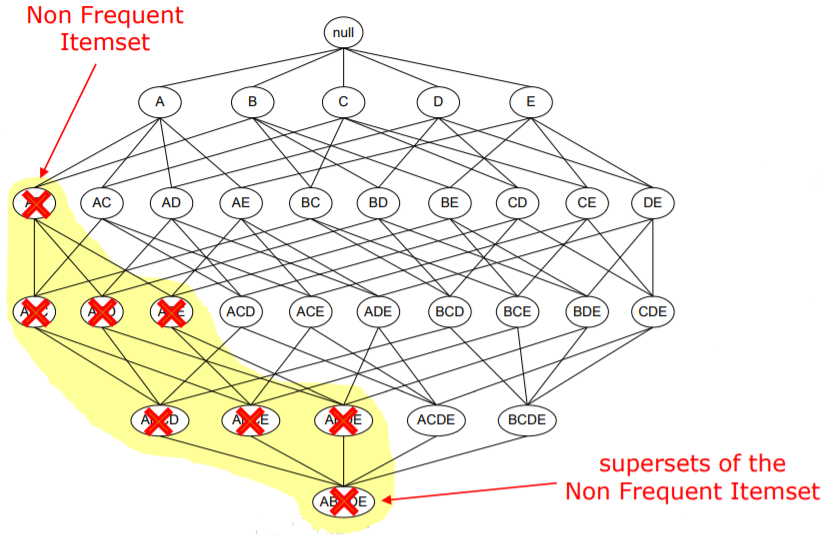
\includegraphics[height=0.5 \linewidth]{association/pict/pruning.png}
	\caption{Esempio di support-based pruning}
\end{figure}

\subsubsection{Algoritmo apriori}
Questo algoritmo genera due operazioni:
\begin{itemize}
	\item \textbf{Candidate Generation}: genera nuovi candidati k-itemset basati su $(k-1)$-itemset frequenti calcolati nella precedente iterazione.
	\item \textbf{Candidate Pruning}: questa operazione elimina alcuni candidati k-itemset usando la strategia del support-based pruning.
\end{itemize}

La complessità computazionale soffre di 4 \textbf{limiti}:
\begin{itemize}
	\item \textit{Support threshold}: se la soglia di supporto è troppo bassa l'albero non viene tagliato molto; questa soglia, però, non deve essere nemmeno troppo elevata altrimenti non vengono considerate potenziali associazioni rilevanti. 
	\item \textit{Numero di item (dimensionalità)}: se il numero di item cresce, c'è bisogno di più spazio in memoria per registrare il support count degli item; inoltre, bisogna considerare anche il costo dell'I/O per passare i dati.
	\item \textit{Numero di transazioni}: l'algoritmo scorre più volte tutta la lista di transazioni, pertanto un numero alto di transazioni inficia sui tempi.
	\item \textit{Average transaction width}: per dataset densi la lunghezza media delle transazioni tende ad essere grande. La massima lunghezza degli itemset frequenti tende ad aumentare; quindi, più sequenze candidate devono essere esaminate durante la generazione e support counting. In aggiunta, aumenta il numero di archi traversi nell'albero durante il support counting.
\end{itemize}

\subsection{Maximal/Closed Frequent Itemsets}
\subsubsection{Rule Generation}
Per ogni k-itemset frequente, Y può generare al limite $2^k-2$ regole di associazione. 

Una regola di associazione può essere estratta partizionando l'itemset Y in 2 sottoinsiemi non vuoti $\{X\}$ e $\{Y-X\}$, tale che $X \rightarrow Y -X$ soddisfa il threshold di confidenza.

\`E molto importante notare che tutte le regole generate da itemset frequenti sono esse stesse frequenti.
\\In pratica, il numero di itemset frequenti prodotti da transazioni possono essere molto grandi. È utile identificare itemset rappresentativi e piccoli con i quali derivare gli itemset grandi; per questo motivo si ragiona in due rappresentazioni:
\begin{enumerate}
	\item Maximal Frequent Itemset
	\item Closed Frequent Itemset
\end{enumerate}

\begin{defn}
	Si definisce \textbf{Maximal Frequent Itemset} un Itemset Frequente per il quale nessuno dei suoi soprainsiemi immediati sono frequenti.
\end{defn}
Nel maximal frequent itemset per ogni nodo si verifica il vincolo della frequenza e si definisce la frontiera dove un nodo non gode più di questa proprietà;  corrisponde alla massima frontiera in cui mi posso spingere.

\begin{figure}[H]
	\centering
	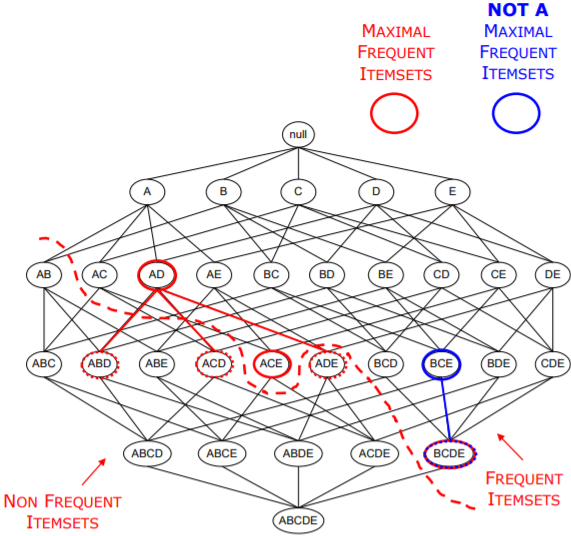
\includegraphics[height=0.7 \linewidth]{association/pict/max_freq_itemset.png}
	\caption{Esempio di frontiera di maximal frequent itemset}
\end{figure}
\textbf{ Un nodo è un Maximal Frequent Itemset se è frequente e se tutte le sue estensioni non sono frequenti.}


\begin{itemize}
	\item Fornisce una rappresentazione compatta dell'insieme di itemset che si sta cercando, la più piccola espressione in cui gli itemset sono derivabili
	\item Calcolato dal più piccolo insieme di itemset dal quale tutti gli itemset frequenti possono essere derivati
	\item È praticabile solo l'algoritmo efficiente usato esplicita la ricerca dei maximal frequent itemset senza numerare tutti i suoi sottoinsiemi
\end{itemize}
Per costruzione \textit{però} non dice la dimensione del supporto rispetto ai suoi sottoinsiemi. In alcuni casi potrebbe servire avere una minima rappresentazione degli itemset frequenti che preservano l'informazione sul supporto.

\begin{defn}
	Si dice che che un itemset X è \textbf{Closed Frequent Itemset} se nessun immediato super-insieme ha esattamente lo stesso support count di X. In ogni caso il suo supporto deve essere $\ge minsup$.
\end{defn}
\`E una grandezza importante quando vi sono gruppi di prodotti venduti a blocco ignorando gli altri.
\\Un esempio è il seguente:
\begin{figure}[H]
	\centering
	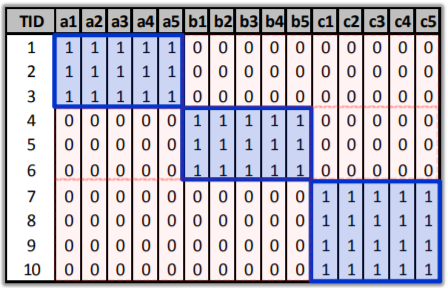
\includegraphics[height=0.5 \linewidth]{association/pict/close_freq_itemset.png}
	\caption{Esempio di gruppi closed frequent itemset}
\end{figure}

Come si può notare in figura, ogni gruppo di variabili (Gruppo A, B e C) è perfettamente associato e non hanno bisogno di mostrare item collegati ad altri gruppi. Assumendo $minsup = 20\%$, il numero totale di itemset frequenti è: $3 \cdot (2^5 -1) = 93$. 
\\In ogni caso vi sono solo 3 closed frequent itemset: 

\[\{a1,a2,a3,a4,a5\}\]

\[\{b1,b2,b3,b4,b5\}\]

\[\{c1,c2,c3,c4,c5\}\]


Questo tipo di itemset sono utili per rimuovere \textbf{regole di associazione ridondanti}. 
\begin{defn}
	Si dice che una regola di associazione $X \rightarrow Y$ è \textbf{ridondante} se esiste un'altra regola $X' \rightarrow Y'$ che rispetta le seguenti proprietà: 
	\begin{itemize}
		\item $X \subseteq X'$
		\item $Y \subseteq Y'$
		\item $s(X \rightarrow Y)  = s(X' \rightarrow Y')$
		\item $c(X \rightarrow Y)  = c(X' \rightarrow Y')$
	\end{itemize}
\end{defn}

Di seguito la gerarchia dei frequent itemset:
\begin{figure}[H]
	\centering
	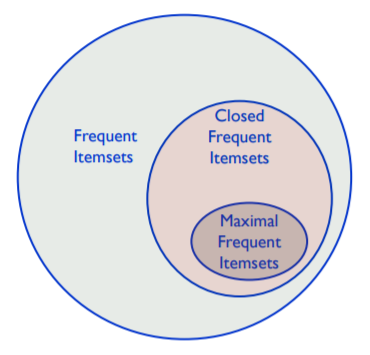
\includegraphics[height=0.45 \linewidth]{association/pict/itemset_freq.png}
	\caption{Gerarchia dei frequent itemset}
\end{figure}

Come si può notare i Maximal Frequent Itemset sono inclusi nei Closed Frequent Itemset perché nessun maximal può avere lo stesso support count del suo immediato superset.

\subsection{Rules Evaluation (*)}
Generati gli insiemi di pattern potenzialmente utili, bisogna ordinarli in base al loro livello di attrattività per il dominio di applicazione. La valutazione della qualità di una regola associativa viene effettuata secondo due criteri:
\begin{itemize}
	\item \textbf{Statistical arguments}: per patterns di items indipendenti e coperti da poche transazioni. Il problema è che \textit{possono catturare relazioni spurie} nei dati, per evitare:
	\begin{itemize}
		\item \textit{Objective Interestingness Measure}: usare statistiche derivate dai dati per determinare quali pattern sono interessanti
		\item \textit{Supporto, confidenza e correlazione}
	\end{itemize}
	\item \textbf{Subjective arguments}: un pattern è considerato non interessante a meno che riveli informazioni inaspettate riguardo ai dati e alla conoscenza:
	\\ \textit{Esmpio:} forte associazione tra acquisto di pannolini e birra. È difficile fare questo tipo di valutazioni, richiede una considerevole quantità di informazioni pregresse dagli esperti di domino.
\end{itemize}

\textit{\`E quindi meglio cercare di applicare un approccio più \textit{oggettivo} alla valutazione: data-driven, indipendente dal dominio in cui si richiede un minimo input dagli utenti (solo dei threshold) e calcolato basandosi sulle frequenze calcolate in una \textbf{Contingency Table}.}
\begin{figure}[H]
	\centering
	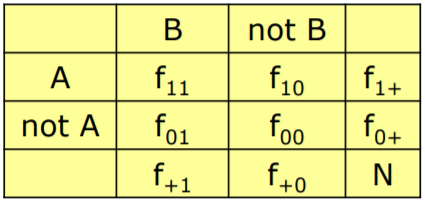
\includegraphics[height=0.2 \linewidth]{association/pict/contingency_table.png}
	\caption{Contingency table}
\end{figure}
Dove:
\begin{itemize}
	\item $f_{1+}$ = support count di A
	\item $f_{+1}$ = support count di B
	\item $N$ = numero di transazioni totali
\end{itemize}
Si assuma che un direttore di un minimarket voglia analizzare la relazione tra le persone che bevono tè e persone che bevono caffè. La seguente contingency table è ottenuta considerando le transazioni disponibili:
\begin{figure}[H]
	\centering
	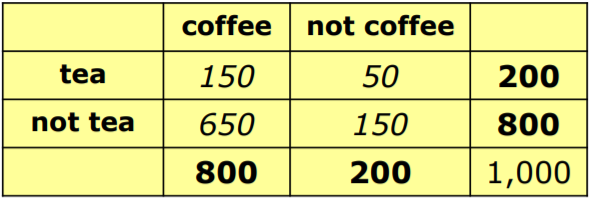
\includegraphics[height=0.2 \linewidth]{association/pict/contingency_table_es.png}
	\caption{Contingency table}
\end{figure}

Si valuti l'associazione: tea $\rightarrow$ coffee, si ottiene:
	 \[support = \frac{f_{11}}{N} = \frac{150}{1000} = 15\%\]
	 \[confidence = \frac{f_{11}}{f_{1+}} = \frac{150}{200} = 75\%\]

Ad una prima occhiata sembrerebbe che le persone che bevono tè tendano a bere anche caffè (vedi confidenza). Si nota, però, che le persone che bevono caffè, a prescindere dal tè sono l'$80\%$ ($\frac{800}{1000}$), mentre la frazione dei bevitori di tè che bevono caffè è solo il $75\%$.

Da questo ragionamento si può concludere che il fatto di bere tè non influisca sulle persone che bevono caffè. Infatti, nonostante l`associazione abbia un alto livello di confidenza ($75\%$), non si può ignorare il supporto dell'itemset conseguente ($80\%$).
Pertanto, vengono definiti altri indici:
\begin{defn}
	Si definisce l'indice \textbf{Lift} il  tasso di confidenza rispetto al supporto del conseguente
	
	\[ Lift = \frac{c(A \rightarrow B)}{s(B)}\]
\end{defn}

\begin{defn}
	Si definisce l'indice \textbf{Interest Factor}, equivalente al Lift ma per attributi binari, in questo modo:
	
	\[ I(A,B)  = \frac{s(A,B)}{s(A)s(B)} = \frac{Nf_{11}}{f_{1+}f_{+1}}\]
\end{defn}
I valori sono così classificati:
\begin{itemize}
	\item $=1$ se A e B sono indipendenti
	\item $>1$ se A e B sono positivamente associati
	\item $<1$ se A e B sono negativamente associati
\end{itemize}
	
\`E molto importante effettuare un' \textbf{analisi di correlazione} (per attributi binari simmetrici): analizza la relazione tra coppie di attributi. Gli attributi continui possono essere analizzati con la correlazione di Pearson; la correlazione per attributi binari è misurata, invece,  usando il $\phi$-coefficient:
\begin{defn}
	Si definisce il \textbf{$\phi$- coefficient} l'espressione che segue:
	\[\phi = \frac{f_{11}f_{00} - f_{01}f_{10}}{\sqrt{f_{1+}f_{+1}f_{0+}f_{+0}}}\]
\end{defn}
Il valore di questo coefficiente varia da $[-1,+1]$. Se gli attributi sono statisticamente indipendenti il valore è $0$.

\begin{defn}
	Si definisce l'indice \textbf{IS Measure} (per attributi binari asimmetrici)	
	\[IS(A,B) = \sqrt{I(A,B)s(A,B)} = \frac{s(A,B)}{\sqrt{s(A)s(B)}}\]
	
	Se A e B sono indipendenti è invece definito come segue:
	
	\[IS(A,B) = \sqrt{s(A)s(B)}\]
	

\end{defn}
Questo indice soffre dello stesso problema della correlazione, il valore può essere grande anche per associazioni incorrelate o negativamente correlate.
Vi sono altri tipi di misure per l'analisi delle relazioni tra coppie di variabili binarie.

\begin{defn}
Una misura \textbf{M} si dice \textbf{Simmetrica} se: $M(A \rightarrow B) = M(B \rightarrow A)$
\end{defn}
\textit{Per come è definito si può quindi dire che l' Interest Factor è una misura simmetrica.}

\begin{defn}
	
Una misura \textbf{M} si dice \textbf{Asimmetrica} se: $M(A \rightarrow B) \ne M(B \rightarrow A)$

\end{defn}
\textit{Per come è definita si può dire che la confidenza è una misura asimmetrica.}
Di seguito la tabella relativa agli indici più utilizzati:

\begin{table}[H]
	\centering
	\begin{tabular}{|p{5cm}|p{5cm}|}
		\hline
		Simmetrico & Asimmetrico \\
		\hline
		Correlazione ($\phi$) & Gini index \\
		Odds ratio & Mutual information \\
		Kappa & Certainty factor \\
		Interest (I) & Added value \\
		Cosine (IS) & J-measure \\
		Jaccard & Goodman-Kruskal \\
		Collective strength & \\
		\hline
	\end{tabular}
\end{table}

È importante capire che ciascuna misura è adatta per analizzare un certo tipo di associazioni come basket market analysis o document analysis. In base al caso bisogna utilizzare gli indici migliori.

\textit{In questa analisi sono stati presentati indici relativi a valutazioni per coppie di attributi binari, ma è possibile estendere l'analisi a più di due attributi usando tabelle delle frequenze in una Contingency Table multi-dimensionale. Gli indici come il Supporto Interest Factor e IS si prestano a questa trattazione.}

\subsection{Simpson's Paradox}

Si consideri la seguente situazione:
\\Un direttore di un mini-market racconta di una curiosa scoperta, legata agli item birra e hot dogs. Una società di consulenza da lui pagata per analizzare i suoi dati di vendita ha scoperto che i clienti che comprano birra sono meno tentati di acquistare hot dogs rispetto a quelli che non acquistano la birra. Il direttore, però, è convinto del contrario, lo sa per esperienza professionale che chi acquista birra tende ad acquistare hot dogs.
\\Come si può risolvere il paradosso?

Si consideri la seguente tabella:
\begin{figure}[H]
	\centering
	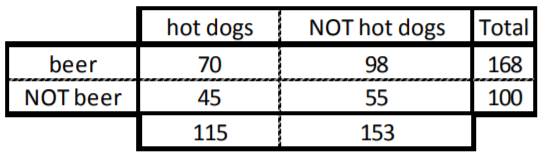
\includegraphics[height=0.2 \linewidth]{association/pict/beer_hotdog.png}
	\caption{Esempio: birra - hot dog}
\end{figure}
Si considerino le seguenti regole con le relative confidenze:
\begin{itemize}
	\item \{beer\} $\rightarrow$ \{hot dogs\} - confidence = $42\%$
	\item \{NOT beer\} $\rightarrow$ \{hot dogs\} - confidence = $45\%$
\end{itemize}	
Da questi numeri si può dedurre che i clienti che acquistano birra sono meno inclini ($42\%$) ad acquistare hot dog rispetto a quelli che non acquistano birra ($45\%$).

Si analizzino gli stessi dati ma categorizzando se il cliente è single o no:
\begin{figure}[H]
	\centering
	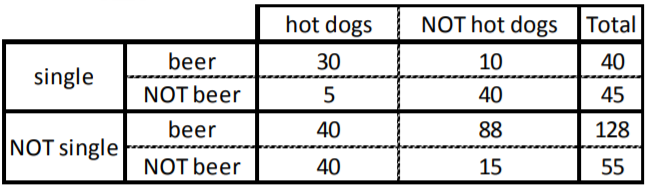
\includegraphics[height=0.2 \linewidth]{association/pict/beer_hotdog_single.png}
	\caption{Esempio: cliente single: birra - hot dog}
\end{figure}
Pertanto si possono derivare queste due coppie di regole:
\begin{itemize}
	\item Single
	\begin{itemize}
		\item \{beer\} $\rightarrow$ \{hot dogs\} - confidence = $75\%$
		\item \{NOT beer\} $\rightarrow$ \{hot dogs\} - confidence = $11\%$
	\end{itemize}
	\item NOT Single
	\begin{itemize}
		\item \{beer\} $\rightarrow$ \{hot dogs\} - confidence = $31\%$
		\item \{NOT beer\} $\rightarrow$ \{hot dogs\} - confidence = $73\%$
	\end{itemize}
\end{itemize}
Da questi dati si può affermare che: i single che acquistano birra sono più inclini ($75\%$) ad acquistare anche hot dog rispetto a quelli che non acquistano birra ($11\%$).
Quindi sia l'azienda di consulenza che il direttore del mini-market avevano ragione soltanto che per comprenderlo bisognava categorizzare i clienti. 

\paragraph{Paradosso di Simpson} (Yule-Simpson effect): è un paradosso della probabilità e statistica, in cui una tendenza appare in diversi gruppi di dati ma sparisce o si inverte quando questi gruppi sono combinati. \\

Bisogna applicare una appropriata stratificazione dei dati per evitare la generazione di associazioni spurie risultati dal paradosso di Simpson. 

Esempio: per i dati del market-basket, la catena di supermercati dovrebbe stratificarli secondo la location del negozio, mentre i dati sanitari da vari pazienti dovrebbero essere stratificati secondo fattori quali l'età o il genere.